\section{Iterators}

\subsection{Iterators}

\begin{frame}
\frametitle{Working with geometries}
	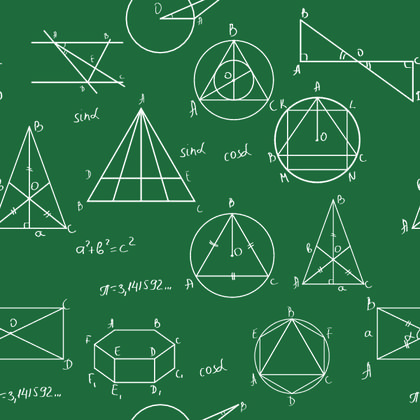
\includegraphics[width=0.7\textwidth]{img/geometries.jpg}
\end{frame}

\subsection{Iterating vertices}
\begin{frame}[fragile]
\frametitle{Iterating vertices}

\begin{lstlisting}[style=pythoncode]
line = QgsGeometry.fromWkt('LINESTRING(1 1, 2 2)')
for vertex in line.vertices():
	print(vertex)
\end{lstlisting}
\pause
\begin{lstlisting}[style=pythonoutput]
<QgsPoint: Point (1 1)>
<QgsPoint: Point (2 2)>
\end{lstlisting}

\end{frame}

\subsection{Iterating parts}
\begin{frame}[fragile]
\frametitle{Iterating parts}

\begin{lstlisting}[style=pythoncode]
multipoint = QgsGeometry.fromWkt('MULTIPOINT((1 1), (2 2), (3 3))')
for point in multipoint.parts():
	print(point)
\end{lstlisting}
\pause
\begin{lstlisting}[style=pythonoutput]
<QgsPoint: Point (1 1)>
<QgsPoint: Point (2 2)>
<QgsPoint: Point (3 3)>
\end{lstlisting}

\end{frame}
